\documentclass[a4paper,11pt]{article}

\usepackage{a4wide}
\usepackage{amsmath}
\usepackage{amssymb}
\usepackage[british]{babel}
\usepackage{graphicx}
\usepackage{listings}
\usepackage{longtable}
\usepackage{prooftree}
\usepackage{synttree}
\usepackage[section]{placeins}

\usepackage{ifthen}

% \todo{Note}. Prints Note in the margin.
\newcommand\todo[1]{
  \-\marginpar[\raggedleft\footnotesize \sf #1]
  {
    \raggedright\footnotesize \sf #1
  }
}

%comment command
\newcommand{\comment}[1]{\begin{quotation} {\sf *** #1 ***} \end{quotation}}

\newcommand{\Bools}{{\mathbb B}}   % set of booleans
\newcommand{\Reals}{{\mathbb R}}   % set of real numbers
\newcommand{\Nats}{{\mathbb N}}    % set of natural numbers
\newcommand{\Natspos}{{\mathbb N^+}} % set of positive natural numbers
\newcommand{\Ints}{{\mathbb Z}}    % set of integer numbers

\newcommand{\Lambdabb}{\Lambda \!\! \Lambda}
% \newcommand{\forallbb}{\forall \!\! \forall}
% \newcommand{\existsbb}{\exists \!\! \exists}
\newcommand{\f}[1]{{\mathit{#1}}}

\newcommand{\true}{\textit{true~}}
\newcommand{\List}{{\mathit{List}}}
\newcommand{\Set}{{\mathit{Set}}}
\newcommand{\Bag}{{\mathit{Bag}}}

\newcommand{\basicsort}{{S_{\mathit{Basic}}}}
\newcommand{\containersort}{{S_{\mathit{Container}}}}
\newcommand{\structsort}{{S_{\mathit{Struct}}}}

% \paragraph{Class name}
% \subparagraph{description}
%
% \subparagraph{superclass of}
%
% \subparagraph{subclass of}
%
% \subparagraph{public methods}
% \begin{description}
%  \item
% \end{description}

\newcommand{\dataclass}[5]{
\begin{flushleft}
\begin{longtable}{p{3cm} p{11cm}}
\multicolumn{2}{c}{\textbf{#1}}\\\hline\hline
\textbf{description} & ~#2~ \\\hline
\textbf{subclass of} & ~#3~ \\\hline
\textbf{superclass of} & ~#4~ \\\hline
\textbf{public methods} & ~#5~ \\\hline
\end{longtable}
\end{flushleft}
}

% \newcommand{\dataclass}[5]{
% \begin{tabular}{ll}
%  \hline
%  \multicolumn{2}{c}{\textbf{#1}} \\\hline \hline
%  \textbf{description} & \mbox{} #2 \mbox{} \\\hline
%  \textbf{subclass of} & \mbox{} #3 \mbox{} \\\hline
%  \textbf{superclass of} & \mbox{} #4 \mbox{} \\\hline
%  \textbf{public methods} & \mbox{} #5 \mbox{} \\\hline
% \end{tabular}
% }

\newtheorem{thdefinition}{Definition}[section]
\newenvironment{definition}
  {\begin{thdefinition}\em}
  {\end{thdefinition}}

\newtheorem{ththeorem}[thdefinition]{Theorem}
\newenvironment{theorem}
  {\begin{ththeorem}\em}
  {\end{ththeorem}}

\newtheorem{thcorollary}[thdefinition]{Corollary}
\newenvironment{corollary}
  {\begin{thcorollary}\em}
  {\end{thcorollary}}

\newtheorem{thlemma}[thdefinition]{Lemma}
\newenvironment{lemma}
  {\begin{thlemma}\em}
  {\end{thlemma}}

\newtheorem{thproperty}[thdefinition]{Property}
\newenvironment{property}
  {\begin{thproperty}\em}
  {\end{thproperty}}

\newtheorem{thexample}[thdefinition]{Example}
\newenvironment{example}
  {\begin{thexample}\em}
  {\end{thexample}}

\newtheorem{thremark}[thdefinition]{Remark}
\newenvironment{remark}
  {\begin{thremark}\em}
  {\end{thremark}}

\newtheorem{thconvention}[thdefinition]{Convention}
\newenvironment{convention}
  {\begin{thconvention}\em}
  {\end{thconvention}}

\newtheorem{thspecification}[thdefinition]{Specification}
\newenvironment{specification}
  {\begin{thspecification}\em}
  {\end{thspecification}}

\newtheorem{thdeclaration}[thdefinition]{Declaration}
\newenvironment{declaration}
  {\begin{thdeclaration}\em}
  {\end{thdeclaration}}

% proof: proof of a theorem
\newenvironment{proof}
  {\textbf{Proof}}
  {\frm{\Box}
   \vspace{1ex}%
  }

\lstdefinelanguage{mcrl2}
{
  morekeywords=[1]{sort, cons, map, var, eqn, act, proc, init, struct},
  morekeywords=[2]{delta, tau},
  morekeywords=[3]{sum, block, allow, hide, rename, comm},
  morekeywords=[4]{Bool, Pos, Nat, Int, Real},
  morekeywords=[5]{List, Set, Bag},
  morekeywords=[6]{true ,false},
  morekeywords=[7]{whr, end, lambda, forall, exists, div, mod, in},
  morekeywords=[8]{contained, TODO, FIXME, XXX},
  sensitive=true,
  morecomment=[l]\%
}[keywords, comments]

\lstset{
  language=mcrl2,
%  basicstyle=\footnotesize,
%  numbers=left,
%  numberstyle=\footnotesize,
%  stepnumber=5,
%  numbersep=5pt
}

\title{Some basic notions concerning the mCRL2 data library}

\author{Jeroen Keiren}

\bibliographystyle{alpha}

\begin{document}

\maketitle

\section{mCRL2}
The language mCRL2 consists of data and processes. The data part contains an equational specification. One can define sorts, functions working upon these sorts, and describe the meaning of these functions by means of equational axioms. The process part contains processes described in the style of CCS, CSP or ACP, with the particular process syntax taken from ACP. It basically consists of a set of uninterpreted actions that may be parametrized with data and time.

\section{The syntax of mCRL2}
See \cite[Appendix B]{groote07dubs}.

\section{Data specification}\label{sec:data_specification}
% Based on discussion with Aad
A data specification consists of a number of \emph{sort}s, a number of \emph{constructor}s for each sort, a number of \emph{map}pings, and a set of \emph{equation}s. A data specification is an equational specification, in which sorts denote types. The semantics of a sort is a set. The elements of the semantics of a sort are described by its constructors, whereas the mappings are functions defined on the semantics of sorts. The equations (axioms) describe equational properties of functions and elements of the semantics. Note that every element of the semantics of a sort can be constructed from its constructors, this is also known as ``no junk''. It may however be the case that an element can be described by several constructors, hence this construction does not satisfy the ``no confusion'' property. The only exception to this are the booleans; \emph{true} and \emph{false} are distinct elements.

% Observe that, when reading equations left-to-right, an equation can be uniquely related to either a constructor or a mapping using the top-level symbol on the left-hand-side of the equation. This property is lost when also allowing the freedom to read the equations right-to-left, such as is done in some provers. Note that it is not necessary for both sides of an equation to include a function symbol as top-level symbol. It may even occur that no function symbol occurs in an equation at all. % According to Muck
% \comment{This could be overcome by also allowing access to the top-level symbol on the right-hand-side.}
%
% Note that functions cannot be uniquely related to sorts, and that equations cannot be uniquely related to functions. % Discussed with Muck

\subsection{Syntax}
We define the syntax that is used to describe data in mCRL2.

\begin{definition}\textbf{(Sort expressions)}
We assume a set of basic sorts $\basicsort$.
Sort expressions $S$ are defined as follows, where $b \in \basicsort$, and $\rightarrow$ is right-associative:
\begin{equation*}
 S ::= \basicsort \shortmid \containersort \shortmid S \times \dots \times S \rightarrow S \shortmid \structsort
\end{equation*}
with $\containersort$ being defined as:
\begin{equation*}
 \containersort ::= \List(S) \shortmid \Set(S) \shortmid \Bag(S)
\end{equation*}
The syntax of structured sorts $\structsort$ is defined as follows (with $p$ a string):
\begin{equation*}
 \structsort ::= p({\it proj}*)?p
\end{equation*}
in which $proj$ has the following syntax:
\begin{equation*}
 {\it proj} ::= S \shortmid p{:}S
\end{equation*}

Structured sorts, with $n \in \Natspos$, $k_i \in \Nats$ with $1 \leq i \leq n$, in general have the following form:
\begin{eqnarray*}
\textbf{struct} & c_1(pr_{1,1}:S_{1,1}, \dots, pr_{1,k_1}:S_{1,k_1})?isc_1\\
              \shortmid & c_2(pr_{2,1}:S_{2,1}, \dots, pr_{2,k_2}:S_{2,k_2})?isc_2\\
              \shortmid & \vdots\\
              \shortmid & c_n(pr_{n,1}:S_{n,1}, \dots, pr_{n,k_n}:S_{n,k_n})?isc_n;
\end{eqnarray*}
We refer to $c_i$ as the constructors of the structured sort. $S_{i,j}$ are the sorts of the arguments of the constructors. $pr_{i,j}$ are names for optional projection functions, retrieving the corresponding argument for a constructor. $isc_i$ are the names of optional recognizer functions, returning a boolean value.
\end{definition}
We call the set  $\containersort$ the container sorts and $S \backslash \{ \basicsort \cup \containersort \cup \structsort \}$ the set of function sorts. In $S_0 \times \dots \times S_n \rightarrow S$ we refer to $S_0, \dots, S_n$ as the domain, and to $S$ as the codomain of the sort.

The language also supports sort aliases like $S_0 = S_1$. In this case only one of the two is treated as a sort, and the other is a reference to it.
\begin{example}\textbf{(Sort aliases)}
 Consider a specification which has $LNat = \List(Nat)$. Now data expressions $x$ of sort $\f{LNat}$ and $x$ of sort $\List(Nat)$ are equivalent.
\end{example}

\begin{definition}\textbf{(Variables)}
We assume a set $V$ of variable names with their associated sorts.
\end{definition}
We write $V_s$ to refer to variables of sort $s$.

\begin{definition}\textbf{(Operations)}
The set of operations $\Omega$ consists of a set of constructors $\Omega_C$ and a set of mappings $\Omega_M$, i.e.
\begin{equation*}
 \Omega = \Omega_C \cup \Omega_M
\end{equation*}
All elements in $\Omega$ can be described, with $n$ a function symbol, and $S$ a sort, as follows
\begin{equation*}
 \Omega ::= n {:} S
\end{equation*}
$\Omega_C$ only contains expressions of the following form.
\begin{equation*}
 \Omega_C ::= n {:} S_B \shortmid n {:} S \times \dots \times S \rightarrow S_B
\end{equation*}
This means that there are only constructors for basic sorts.
\end{definition}
In the remainder we write $\Omega_{C,s}$ to denote the constructors of sort $s$. That is those $n$ in $\Omega_C$ with codomain $s$.

\begin{definition}\textbf{(Data expressions)}
We inductively define data expressions $e$, with sort expressions $S$ and variables $x$ as follows:
\begin{eqnarray*}
 e & ::= & x \shortmid n \shortmid e(e, \dots, e) \shortmid \lambda x{:}S, \dots, x{:}S . e \shortmid \forall x{:}S, \dots, x{:}S . e \shortmid \exists x{:}S, \dots, x{:}S . e \\
   & \shortmid & e \textbf{ whr } x = e, \dots, x = e \textbf{ end} \shortmid \{x{:}S \mid e\}
\end{eqnarray*}
Here $e(e, \dots, e)$ denotes application of data expressions, $\lambda x{:}S, \dots, x{:}:S . e$ denotes abstraction. $\forall x{:}S, \dots, x{:}S . e$ and $\exists x{:}S, \dots, x{:}S . e$ describe universal and existential quantification. $\{x{:}S \mid e\}$ denotes set or bag comprehension. Note that in the remiander we will write $\Lambda$ to denote any binding operator when describing rules that apply to all binding operators, i.e. $\lambda$, $\exists$, $\forall$, $\{\}$.
\end{definition}

% \begin{convention}\textbf{(Quantifiers)}
% We write $\forall x_0{:}s_0, \dots, x_n{:}s_n . t$ as shorthand for $\forall(\lambda x_0{:}s_0, \dots, x_n{:}s_n . t)$ and $\exists x_0{:}s_0, \dots, x_n{:}s_n . t$ for $\exists(\lambda x_0{:}s_0, \dots, x_n{:}s_n . t)$.
% \end{convention}
% 
\begin{convention}\textbf{(System defined operators)}
We write system defined operators as infix operators, hence we write $b_1 \land b_2$ for $and(b_1,b_2)$, etc. For system defined operators we also have a notion of operator precedence. See Section~\ref{sec:predef_sorts} for a complete overview of system defined sorts.
\end{convention}
% 
% \comment{Add infix conventions for other system defined sorts}
% 
% \begin{convention}\textbf{(Where-clause)}
% We write $t \textbf{ whr } x_0 = t_0, \dots, x_n = t_n \textbf{ end}$ as shorthand for $(\lambda x_0, \dots, x_n . t)(t_0, \dots, t_n)$.
% \end{convention}
% 
% \begin{convention}\textbf{(Set/Bag comprehension)}
%  We write $\{ x{:}s | t \}$ as shorthand for $@Set(\lambda x{:}s . t)$ if $t$ is of sort $\Bools$. When $t$ is of sort $\Nats$ we treat this as a shorthand for $@Bag(\lambda x{:}s . t)$.
% \end{convention}
% 
% \begin{convention}\textbf{(Set enumeration)}
%  We write $\{ t_0, \dots, t_n \}$ as shorthand for $\{ x \shortmid x \approx t_0 \lor \dots \lor x \approx t_n \}$. This is called set enumeration.
% \end{convention}
% 
% \begin{convention}\textbf{(Bag enumeration)}
%  We write $\{ t_0:m_0, \dots, t_n:m_n \}$ as shorthand for $\{ x | \mathit{if}(x \approx t_0, m_0, \mathit{if}(x \approx t_1, m_1, \dots \mathit{if}(t_n, m_n, 0) \dots )) \}$. This is called bag enumeration.
% \end{convention}

\begin{definition}\textbf{(Signature)}
A signature $\Sigma$ is a structure $(\basicsort, \Omega)$, where $\basicsort$ is a set of sorts and $\Omega$ is a set of operations. $\basicsort$ contains at least $\Bools, \Natspos, \Nats, \Ints, \Reals$.
\end{definition}

We now define the validity of data expressions with a number of syntax-directed derivation rules.
\begin{definition}\textbf{(Valid data expressions)}
We assume a context $\Gamma$, which is a set of typing statements of variables and operations used in the typing derivations. Note that we write $\Gamma, x{:}s$ as shorthand for $\Gamma \cup \{ x{:}s \}$ and $\exists^1_s$ to denote that there is \emph{exactly one} such $s$.

\begin{tabular}{cc}
~\\
\begin{prooftree}
 x {:} s \in \Gamma
 \justifies
 \Gamma \vdash x {:} s
 \using (\f{Var})
\end{prooftree}
&
\begin{prooftree}
 n {:} s \in \Gamma
 \justifies
 \Gamma \vdash n {:} s
 \using (\f{Op})
\end{prooftree}
\\~&\\
\multicolumn{2}{c}{
\begin{prooftree}
 \Gamma, x_0 {:} s_0, \dots, x_n {:} s_n \vdash e {:} s
 \justifies
 \Gamma \vdash (\lambda x_0 {:} s_0, \dots, x_n {:} s_n . e) {:} s_0 \times \dots \times s_n \rightarrow s
 \using (\f{Abs})
\end{prooftree}
}
\\~&\\
\multicolumn{2}{c}{
\begin{prooftree}
 \exists^1_{s0, \dots, s_n} (
   \Gamma \vdash t {:} s_0 \times \dots \times s_n \rightarrow s
   \quad
   \Gamma \vdash t_0 {:} s_0
   \quad
   \dots
   \quad
   \Gamma \vdash t_n {:} s_n
 )
 \justifies
 \Gamma \vdash t(t_0, \dots, t_n) {:} s
 \using (\f{Appl})
\end{prooftree}
}
\\~&\\
\multicolumn{2}{c}{
\begin{prooftree}
 \exists^1_{s_0, \dots, s_n} (
 \Gamma \vdash x_1{:}s_1
 \quad
 \Gamma \vdash e_1{:}s_1
 \quad
 \dots
 \quad
 \Gamma \vdash x_n{:}s_n
 \quad
 \Gamma \vdash e_n{:}s_n
 \quad
 \Gamma, x_0 {:} s_0, \dots, x_n {:} s_n \vdash e {:} s
 )
 \justifies
 \Gamma \vdash (e \textbf{ whr } x_0 = e_0, \dots, x_n = e_n \textbf{ end}) {:} s
 \using (\f{Where})
\end{prooftree}
}
\\~&\\
\begin{prooftree}
 \Gamma, x_0 {:} s_0, \dots, x_n {:} s_n \vdash e {:} \Bools
 \justifies
 \Gamma \vdash (\forall x_0 {:} s_0, \dots, x_n {:} s_n . e) {:} \Bools
 \using (\f{Forall})
\end{prooftree}
&
\begin{prooftree}
 \Gamma, x_0 {:} s_0, \dots, x_n {:} s_n \vdash e {:} \Bools
 \justifies
 \Gamma \vdash (\exists x_0 {:} s_0, \dots, x_n {:} s_n . e) {:} \Bools
 \using (\f{Exists})
\end{prooftree}
\\~&\\
\begin{prooftree}
 \Gamma, x {:} s \vdash e {:} \Bools
 \justifies
 \Gamma \vdash \{ x {:} s \mid e \} {:} \Set(s)
 \using (\f{SetComp})
\end{prooftree}
&
\begin{prooftree}
 \Gamma, x {:} s \vdash e {:} \Nats
 \justifies
 \Gamma \vdash \{ x {:} s \mid e \} {:} \Bag(s)
 \using (\f{BagComp})
\end{prooftree}
\\~&\\
\end{tabular}
\end{definition}


The $\Sigma$-algebra is characterized by means of equational logic. We describe the syntax of formulae in the equational logic.
\begin{definition}\textbf{(Equations)}
Consider data expressions $e$, the syntactic set of equations adheres to
\begin{equation*}
 E ::= e = e \shortmid e \rightarrow e = e
\end{equation*}
\end{definition}

We also introduce two rules for validity of equations.

\begin{tabular}{cc}
~&\\
\begin{prooftree}
 \exists^1_s(
  \Gamma \vdash d {:} s
  \quad
  \Gamma \vdash e {:} s
 )
 \justifies
 \Gamma \vdash d = e
 \using (\f{Eq})
\end{prooftree}
&
\begin{prooftree}
 \Gamma \vdash c : \Bools
 \quad
 \exists^1_s(
  \Gamma \vdash d {:} s
  \quad
  \Gamma \vdash e {:} s
 )
 \justifies
 \Gamma \vdash c \rightarrow d = e
 \using (\f{CondEq})
\end{prooftree}
\\~&
\end{tabular}

\begin{definition}\textbf{(Data specification)}
A data specification consists of sorts, constructors, mappings and equations, i.e.
\begin{equation*}
 D = (S, \Omega, E)
\end{equation*}
\end{definition}

\subsection{Semantics}
\begin{definition}\textbf{($\Sigma$-Algebra)}
A $\Sigma$-algebra $A$ assigns meaning to signature $\Sigma = (\basicsort, \Omega)$ by assigning a carrier set $A(s)$ to each sort $s$. $A(s)$ is the set containing the elements of sort $s$. Furthermore it assigns a total function $A(n {:} s)$, yielding an element of sort $A(s)$, to each operation $n {:} s \in \Omega$. We write $A(n)$ for $A(n {:} s)$ when $s$ is clear from the context.

Note that all elements from carrier set $A(s)$ can be obtained from the constructors $n {:} s \in \Omega_C$.
\end{definition}

\begin{example}
Suppose we have a signature $\Sigma = (\basicsort, \Omega)$, with
\begin{eqnarray*}
\basicsort & = & \{ {\it Nat} \}\\
\Omega_C & = & \{ zero{:}{\it Nat}, succ{:}{\it Nat} \rightarrow {\it Nat} \}\\
\Omega_M & = & \{ add {:} {\it Nat} \times {\it Nat} \rightarrow {\it Nat} \}
\end{eqnarray*}
We give semantics to this by $\Sigma$-algebra $A$, where:
\begin{eqnarray*}
 A({\it Nat})                                             & = & \Nats \\
 A({\it Nat} \rightarrow {\it Nat})                       & = & \Nats \rightarrow \Nats \\
 A({\it Nat} \times {\it Nat}) \rightarrow {\it {\it Nat}} & = & \Nats \times \Nats \rightarrow \Nats \\
 A(zero)                          & = & 0 \\
 A(succ)                          & = & \lambda n {:} \Nats . (n + 1) \\
 A(add)                           & = & \lambda m, n {:} \Nats \times \Nats . (m + n)
\end{eqnarray*}
\end{example}

All elements of a carrier set $A(s)$ of sort $s$ can be obtained by inductively applying the constructors $n : s \in \Omega_C$ of $s$. This process is referred to as \emph{enumeration}. Note that this requires all elements of other sorts $s' \in S$ that occur as subexpression in $s$.
\begin{example}
As an example of obtaining all elements of a sort from its constructors, let us again look at the natural numbers $Nat$. We take a data expression representing a natural number $n$, which according to the constructors of $Nat$ could be either $0$ or $succ(n')$---the successor of another natural number. We repeat this process for $n'$, and continue this way until all variables have been eliminated. A tree representation of this is given in Figure \ref{fig:enum_tree}. Note that this process does not necessarily terminate.
\end{example}

\begin{figure}[htp]
\begin{center}
\synttree[ $n$
           [$0$]
           [$succ(n')$
             [$succ(0)$]
             [$succ(succ(n''))$
               [ $succ(succ(0))$ ]
               [ \dots ]
             ]
           ]
         ]
\caption{Enumeration of natural numbers using $0$ and $succ$}
\label{fig:enum_tree}
\end{center}
\end{figure}

\subsubsection{Variables and data expressions}
In order to define the semantics of data expressions, we introduce the notion of assignment. Using $V_s$ to denote the variables of sort $s$ from $V$, an assignment of a set of variables $V$ for a $\Sigma$-algebra $A$ ($\alpha : V \rightarrow A$) is a family $\alpha = (\alpha_s)_{s \in S}$ of total functions $\alpha_s : V_s \rightarrow A(s)$.

A meaning is given to a data expression $e$ over a signature $\Sigma$ extended with variables $V$---in short $e \in T_{\Sigma(V)}$---using a $\Sigma$-algebra $A$ and an assignment $\alpha$. It is called the value of $e$ for $\alpha$ and is denoted by $A(\alpha)(e)$. In the sequel we also write $e \in T_{\Sigma(V),s}$ to denote the data expressions over signature $\Sigma$ and variables $V$ of sort $s$. With $\Lambdabb$ we denote abstraction in the semantic domain.
\begin{definition}
We define the notion of value inductively on the structure of $e$:
\begin{itemize}
 \item $A(\alpha)(x) = \alpha_s(x)$, where $x \in V_s$ and $s \in S$;
 \item $A(\alpha)(n) = A(n)$; %\alpha(\omega)$, where $\omega = n {:} s \in \Omega$;
 \item $A(\alpha)(e(u_0, \dots, u_n)) = A(\alpha)(e)(A(\alpha)(u_0), \dots, A(\alpha)(u_n))$ where $e \in T_{\Sigma(V),s_0 \times \dots \times s_n \rightarrow s}$ and $u_i \in T_{\Sigma(V),s_i}$
 \item $A(\alpha)(\Lambda x_0{:}s_0, \dots, x_n{:}s_n . e) = \Lambdabb d_0 \in A(s_0), \dots d_n \in A(s_n) . A(\alpha[x_i := d_i]_{0 \leq i \leq n})(e)$
\item $A(\alpha)(e \textbf{ whr } x_0 = e_0, \dots, x_n = e_n \textbf{ end} = A(\alpha[x_i := d_i]_{0 \leq i \leq n})(e) \textbf{ where } d_0 \in A(s_0) = A(\alpha)(e_0), \dots d_n \in A(s_n) = A(\alpha)(e_n) \textbf{ end}$
\end{itemize}
\end{definition}

We introduce the syntactic notion of substitution. For a signature $\Sigma = (S, \Omega)$ and associated sets of variables $V$ and $W$, a substitution is a family $\sigma = (\sigma_s)_{s \in S}$ of functions $\sigma_s : V_s \rightarrow T_{\Sigma(W),s}$. We denote this by $\sigma : V \rightarrow T_{\Sigma(W)}$.
\begin{definition}\textbf{(Substitution)}
We define the application of a substitution $\sigma$ to a data expression inductively as follows:
\begin{itemize}
 \item $\sigma(x) = \sigma_s(x)$, where $x \in V_s$ and $s \in S$
 \item $\sigma(n) = n$, where $n : S \in \Omega$
 \item $\sigma(e(u_0, \dots, u_n)) = \sigma(e)(\sigma(u_0), \dots, \sigma(u_n))$
 \item $\sigma(\Lambda x_0, \dots, x_n . e) = \Lambda y_0, \dots, y_n . \sigma[x_i:=y_i]_{0 \leq i \leq n}(e)$, if $y_i$ does not occur free in $e$ and $\sigma(y_i) = y_i$ (for all $0 \leq i \leq n$)
 \item $\sigma(e \textbf{ whr } x_0 = e_0, \dots, x_n = e_n \textbf{ end}) = \sigma[x_i := y_i]_{0 \leq i \leq n}(e) \textbf{ whr } y_0 = \sigma(e_0), \dots, y_n = \sigma(e_n)$, if $y_i$ does not occur free in $e$ and $\sigma(y_i) = y_i$ (for all $0 \leq i \leq n$)
\end{itemize}
\end{definition}

\begin{remark}
There is a close relation between the syntactic notion of substitution and the semantic notion of assignment. Assignments may simulate substitutions. For all signatures $\Sigma$, associated sets of variables $V, W$, substitutions $\sigma : V \rightarrow T_{\Sigma(W)}$, $\Sigma$-algebras $A$, assignments $\beta : W \rightarrow A$, and data expressions $e \in T_{\Sigma(V)}$, we have:
\begin{equation*}
 A(\beta)(\sigma(e)) = A(\alpha)(e)
\end{equation*}
where assignment $\alpha : V \rightarrow A$ is defined by $\alpha(x) = A(\beta)(\sigma(x))$, for all $x~\in~V$.
\end{remark}

\subsubsection{Equational logic}
The semantics of a formula in equational logic is expressed by a satisfaction relation.
\begin{definition}\textbf{(Satisfaction relation)}
For a $\Sigma$-algebra $A$, a condition $c~\in~T_{\Sigma(V),\Bools}$, a sort $s \in S$ and data expressions $d, e~\in~T_{\Sigma(V),s}$, the satisfaction relation $\vDash_{EL}$ is defined by:
\begin{equation*}
 A \vDash_{EL} c \rightarrow d = e~\text{iff $A(\alpha)(d) = A(\alpha)(e)$ and $(A(\alpha)(c) = true)$, for all assignments $\alpha : V \rightarrow A$}
\end{equation*}
\end{definition}
If $A \vDash_{EL} c \rightarrow d = e$, we say that $d = e$ is valid in $A$. If $c$ is omitted, we consider it to be $true$.

\begin{definition}\textbf{(Model)}
For a set of equations $E \subseteq EL(\Sigma)$, a $\Sigma$-algebra $A$ is called a model of $E$ if $A \vDash_{EL} eq$, for all $eq \in E$.
\end{definition}
We denote the class of all models of $E$ as $Mod_{EL}(E)$.

\begin{definition}\textbf{(Logical consequence)}
An equation $eq \in EL(\Sigma)$ is called a logical consequence of a set of equations $E$, iff $eq$ is valid in all models of $E$, denoted $E \vDash_{EL} eq$. That is
\begin{equation*}
 E \vDash_{EL} eq~\text{iff}~A \vDash_{EL} eq,~\text{for all}~A \in Mod_{EL}(E)
\end{equation*}
\end{definition}

\subsubsection{Data specification}
In mCRL2 the set of basic sorts $\basicsort$ is obtained by those sorts preceded with the \lstinline{sort} keyword. Function sorts may be used implicitly in the specification. The constructor functions $\Omega_C$ are those functions preceded be the \lstinline{cons} keyword. The mappings $\Omega_M$ are preceded by \lstinline{map}. Finally, the equations $EL(\Sigma)$ are preceded by \lstinline{eqn}.

\subsection{Some notions on sorts}\label{sec:sort_notions}
\subsubsection{Finiteness}\label{sec:sort_finiteness}
For some applications it is interesting to know whether sort is finite.

Let function $\f{DependentSorts}: \Omega_C \rightarrow 2^S$, that obtains the sorts on which a constructor depends, be defined inductively as:
\begin{equation*}
 \f{DependentSorts}(n{:}s) = \begin{cases}
             \emptyset & \text{if $s \in \basicsort$}\\
             \bigcup_{0 \leq i \leq n}(\{ s_i \} \cup \f{Sorts}(s_i)) & \text{if $s = s_0 \times \dots \times s_n \rightarrow s'$}
            \end{cases}
\end{equation*}

Let the function $\f{Sorts}: S \rightarrow 2^S$, that obtains the sorts on which its argument depends, be defined recursively as:
\begin{equation*}
 \f{Sorts}(s) = \begin{cases}
             \bigcup_{n \in \Omega_{C,s}} \f{DependentSorts}(n) & \text{if $s \in \basicsort$}\\
             \f{Sorts}(s') & \text{if $s \in \containersort$}\\
             \bigcup_{0 \leq i \leq n} \f{Sorts}(s_i) \cup \{ s' \} & \text{if $s = s_0 \times \dots \times s_n \rightarrow s'$}\\
             \bigcup_{0 \leq i \leq n} \bigcup_{0 \leq j \leq m_i} \f{Sorts}(s_{i,j}) & \text{if $s = \textbf{struct } c_i(pr_{i,1}{:}s_{i,1}, \dots, pr_{i,m_i}{:}s_{i,m_i})?isc_i$}\\&\text{\indent for $0 \leq i \leq n, 1 \leq j \leq m_i$}
            \end{cases}
\end{equation*}

We inductively define predicate $\f{Finite}: S \rightarrow \Bools$ as follows:
\begin{equation*}
 \f{Finite}(s) = \begin{cases}
              \Omega_{C,s} \neq \emptyset \land s \not \in \f{Sorts}(s) & \\\indent \land (\forall n \in \Omega_{C,s}:\\\indent (\forall s' \in \f{DependentSorts}(n): \f{Finite}(s'))) & \text{if $s \in \basicsort$}\\
              \f{Finite}(s') & \text{if $s = \Set(s')$} \\
              \f{false} & \text{if $s \in \containersort$ and $s \neq \Set(s')$ for all $s'$}\\
              (\forall i: \f{Finite}(s_i)) \land \f{Finite}(s') & \text{if $s = s_0 \times \dots \times s_n \rightarrow s'$}\\
              s \not \in \f{Sorts}(s) \land (\forall s' \in \f{Sorts}(s): \f{Finite}(s'))) & \text{if $s = \textbf{struct } c_i(pr_{i,1}{:}s_{i,1}, \dots, pr_{i,m_i}{:}s_{i,m_i})?isc_i$}\\&\text{\indent for $0 \leq i \leq n, 1 \leq j \leq m_i$}
             \end{cases}
\end{equation*}

\subsubsection{Equivalence of sorts}
\comment{To be defined}

\subsection{Some notions on data expressions}
\begin{definition}\textbf{(Free variables)}
We inductively define the set of free variables $FV(e)$ of a data expression $e$ as follows:
\begin{eqnarray*}
FV(x) & = & \{ x \}\\
FV(n) & = & \emptyset\\
FV(e(e_0, \dots, e_n)) & = & FV(e) \cup \bigcup_{0 \leq i \leq n} FV(e_i)\\
FV(\lambda x_0{:}s_0, \dots, x_n{:}s_n . e) & = & FV(e) \setminus \{ x_i \shortmid 0 \leq i \leq n \}
\end{eqnarray*}
\end{definition}

\begin{definition}\textbf{(Closed)}
We say that a data expression $e$ is closed iff $FV(e) = \emptyset$.
\end{definition}

\section{Predefined sort specifications}\label{sec:predef_sorts}
% Retrieved from the RADV lecture notes
mCRL2 provides a number of predefined sorts. For an overview of these sorts, with the full specifications that are generated see \cite[Appendix A]{groote07dubs}.
\comment{To be copied from the book}

\section{Type checking}
In mCRL2 types are only made explicit in function declarations and abstractions. For places where type information is not explicitly included these can be inferred by a type-checking algorithm if the specification is typable. This algorithm attempts to infer the types of expressions in the program from their contexts. Type checking is outside the scope of this document.

\subsection{Type conversion rules}
% List of casts obtained from struct.h
The toolset supports a number of convenience functions \texttt{A2B} in order to cast numeric types. In this $A \neq B$, and $A,B \in \{Pos, Nat, Int, Real \}$. Of these, the type checker only uses upcasts, e.g. \texttt{Pos2Nat}.

\section{Rewriting}
The rewriters used in mCRL2 \cite{weerdenburg2007} take the equations as defined in the data specification and interpret these from left to right as rewrite rules. A rewrite rule means that an expression matching the left hand side of this rule may be rewritten to the right hand side of the rule. Additionally, a rewrite rule may be equipped with a condition, such that an expression is only rewritten if the condition holds. Such rewrite rules are referred to as conditional rewrite rules.

Rewriting of a data expression is done by repeatedly applying rewrite rules until a normal form is reached, that is, until no rewrite rules can be applied to the expression. Note that the mCRL2 toolset supports multiple rewrite strategies, which do not have the same termination conditions. However, whenever the rewrite system derived from the data specification is terminating, the rewriters will also terminate.

Rewriting is a purely syntactic manipulation. Given a set of rewrite rules a normal form for a data expression is returned. If two expressions have the same normal form, they are considered equal.

In rewriting we can parametrize a rewriter with a set of substitutions which are performed during rewriting. This is mostly for performance reasons.

We consider a rewrite system $R$.
\begin{definition}\textbf{(Rewrite step)}
There is a rewrite step $t \rightarrow_R u$ if there is a position $\pi$ (of a subterm of $t$), a rewrite rule $l \rightarrow r$ in $R$ and a substitution $\sigma$, such that $t|\pi = \sigma(l)$ and $u = t[\pi](\sigma(r))$, with $t|\pi$ the subterm of $t$ at position $\pi$, and $t[\pi]u$ is $t$ with its subterm at position $\pi$ replaced by $u$.
\end{definition}

\begin{definition}\textbf{(Normal form)}
At term $t$ is in normal form when there is no rewrite step $t \rightarrow_R u$.
\end{definition}

\begin{definition} \textbf{(Rewrite sequence)}
A rewrite sequence $t \twoheadrightarrow_R u$ is a sequence of rewrite steps, such that $t \twoheadrightarrow_R v$ and $v \rightarrow_R u$.
\end{definition}

\begin{definition}\textbf{(Normal forms of a term)}
The normal forms of a term $t$ are those terms that occur as the last term in a rewrite sequence starting with $t$.
\end{definition}

%We define $match$ as the function which gives a rewrite rule with its variables instantiated, if such a rewrite rule can be found and its condition is satisfied. Note that we interpret conditions as equations with the right or left hand side implicitly set to true, and a condition $c$ is satisfied iff $c = true$ holds.

% Let $x, x_0, \dots x_n$ be variables, $n$ an arbitrary function symbol, $e, e_0, \dots, e_n$ arbitrary terms. A rewriter $R$ returns a normal form, which can be characterized as follows. Note that we explicitly do not characterize the order in which rewriting is performed, as this is strategy dependent.
% \begin{eqnarray*}
% R(x) & = & \begin{cases} \text{$e'$ if $match(x) \equiv x = e'$} \\
%                          \text{$x$ otherwise}
%            \end{cases}\\
% R(n) & = & \begin{cases} \text{$e'$ if $match(n) \equiv n = e'$} \\
%                          \text{$n$ otherwise}
%            \end{cases}\\
% R((\lambda x_0{:}s_0, \dots x_n{:}s_n . e)(e_0, \dots, e_n)) & = & R(e[x_0:= e_0]\dots[x_n := e_n]) \\
% R(e(e_0, \dots, e_n)) & = & \begin{cases} \text{$e'$ if $match(e(e_0, \dots, e_n)) \equiv e(e_0, \dots, e_n) = e'$}\\
%                                           \text{$R(e)(R(e_0), \dots, R(e_n))$ otherwise}
%                             \end{cases}\\
% R(e \textbf{ whr } x_0 = e_0, \dots, x_n = e_n) & = & R(e[x_0 := e_0]\dots[x_n := e_n])
% \end{eqnarray*}
% This procedure is applied repeatedly until a normal form is reached.
% 
% Additionally we can define rules for abstraction. These should not be applied repeatedly, as this might lead to non-termination, because the result of executing such a rewrite rule again satisfies the lefthandside of the same rule. \footnote{Testing shows that it is not a regression with respect to the current setting of rewrite rules to leave these out}
% \begin{eqnarray*}
% R(\Lambda x_0{:}s_0, \dots x_n{:}s_n . e) & = & \lambda x_0{:}s_0, \dots x_n{:}s_n . R(e)\\
% \end{eqnarray*}
% 
% We can extend this approach with substitutions, such that substitutions are carried out during rewriting. This is fairly straightforward. We do however need to take care that we avoid capture in the case that binding is used. Let $x, x_0, \dots x_n$ be variables, $n$ an arbitrary function symbol, $t, t_0, \dots, t_n$ arbitrary terms. Furthermore, assume that variables $y_i, (0 \leq i \leq n)$ are fresh for their context. We define a rewriter $R$ with substitution $\sigma$ as follows:
% \begin{eqnarray*}
% R(x, \sigma) & = & \begin{cases} \text{$e'$ if $match(\sigma(x)) \equiv \sigma(x) = e'$} \\
%                                  \text{$\sigma(x)$ otherwise}
%                    \end{cases}\\
% R(n, \sigma) & = & \begin{cases} \text{$e'$ if $match(n) \equiv n = e'$} \\
%                                  \text{$n$ otherwise}
%                    \end{cases}\\
% R((\lambda x_0{:}s_0, \dots x_n{:}s_n . e)(e_0, \dots, e_n), \sigma) & = & R(e[x_0:= y_0]\dots[x_n := y_n], \sigma[y_0 := e_0], \dots, y_n := e_n]) \\
% R(e(e_0, \dots, e_n), \sigma) & = & \begin{cases} \text{$e'$ if $match(\sigma(e(e_0, \dots, e_n))) \equiv \sigma(e(e_0, \dots, e_n)) = e'$}\\
%                                                   \text{$R(e, \sigma)(R(e_0, \sigma), \dots, R(e_n, \sigma))$ otherwise}
%                             \end{cases}\\
% R(e \textbf{ whr } x_0 = e_0, \dots, x_n = e_n, \sigma) & = & R(e[x_0 := y_0]\dots[x_n := y_n], \sigma[y_0 := e_0]\dots[y_n := e_n])
% \end{eqnarray*}
% 
% Again we can additionally define rules for abstraction in a similar fashion as before.
% \begin{eqnarray*}
% R(\Lambda x_0{:}s_0, \dots x_n{:}s_n . e, \sigma) & = & \Lambda y_0{:}s_0, \dots y_n{:}s_n . R(e[x_0 := y_0]\dots[x_n := y_n], \sigma)
% \end{eqnarray*}

\section{Proving}
Proving is, like rewriting, a syntactic operation. However, where in rewriting the equations are only interpreted left to right, the provers use the equations to their full extent. The provers determine whether or not an expression of sort Bool is a tautology or a contradiction. An in depth discussion of a prover for mCRL2 is presented by Luc Engelen \cite{engelen2006}.

\section{Equality checking}
In practice a lot of equality checking is performed, for example for evaluating conditions in rewriters. In its basic form, the question is merely whether two terms are equal. In addition, like in rewriting, substitutions may be provided to check whether to terms are equal under a certain substitution. This is again for performance reasons. Checking for equality can be performed by a rewriter as well as by a prover.

The requirements for an equality checker $Eq$ are as follows:
\begin{eqnarray*}
 Eq({\it true}, {\it false}) & \equiv & {\it false}\\
 Eq(e, e')                   & \implies & e = e'
\end{eqnarray*}
Thus, \textit{true} and \textit{false} are different, and if two terms are said to be equal, they are indeed equal.

\section{Enumeration}
Let $range(e)$ be the set of all possible values that data expression $e$ can attain. A sort $S$ is \emph{enumerable} iff a function $enum_S$ exists that maps an arbitrary data expression $e$ of sort $S$ to a finite set of closed data expressions $\{ e_1, \dots, e_k \}$, such that $range(e) = \bigcup_{i=1}^{k} range(e_i)$. By repeatedly applying $enum_S$ to non-constant data expressions $x_i$, a tree expansion of the data expression is obtained. The leafs of this tree form a finite representation of the data expression. For data expressions of finite sort, this tree is always finite as well.

\section{Mapping an data specification to the signature}
In this section we map the current implementation of a data specification to the signature as described in this document.

\subsection{Details of the current implementation}
We now map parts of the current (procedural style) implementation in the mCRL2 toolset to the signature as described above. This is the implementation directly built upon the ATerm library.

\subsubsection{Sort expressions}
\begin{description}
 \item [Sort expressions] are the \emph{sort expressions} $S$. Internally referred to as \texttt{SortExpr}. Note that Sort identifiers, Arrow sorts, Sort references, Structured sorts and Container sorts are all sort expressions.
 \item [Sort identifiers] are the basic sorts $S_B$. Internally referred to as \texttt{SortId}.
 \item [Arrow sorts] are the function sorts $S \backslash \{ \basicsort \cup \containersort \}$. Internally referred to as \texttt{SortArrow}.
 \item [Sort references] are the aliases $S_0 = S_1$. Internally referred to as \texttt{SortRef}.
 \item [Container sorts] are the $\List(S)$, $\Set(S)$ and $\Bag(S)$ sorts. Internally these are referred to as \texttt{SortCons(Constructor type, SortExpr)}, in which \texttt{SortExpr} denotes the element sort, and \texttt{Constructor type} is one of \texttt{SortList, SortSet, SortBag} to denote List, Set and Bag sorts respectively.
 \item [Structured sorts] are the $Struct(S)$ sorts. Internally these are referred to as \texttt{SortStruct(StructCons+)}, in which \texttt{StructCons+} is a non-empty list of constructors. A constructor has the form \texttt{StructCons(Name, StructProj*, Recogniser?)}. In this, \texttt{Name} represents the name of the constructor (a string), \texttt{Recogniser?} represents the name of the recogniser function for this constructor, which may be $nil$ to denote that there is no recogniser. \texttt{StructProj*} is a (possibly empty) list of expressions that denotes the arguments of the constructor, with their optional projection functions. An expression for an argument has the following form: \texttt{StructProj(Name?, SortExpr)}, in this \texttt{Name?} denotes the name of the argument, which is either a string or $nil$ denoting that the argument has no name. \texttt{SortExpr} denotes the sort of the argument.
\end{description}

\subsubsection{Data expressions}
\begin{description}
 \item[Data expressions] are the data expressions. Internally referred to as \texttt{DataExpr}.
 \item[Data variable] is a variable of a certain sort. Corresponding to the first case above. Internally referred to as \texttt{DataVarId}.
 \item[Data operation] is a function with its sort, an element of $\Omega$ as in the second case above. Internally referred to as \texttt{OpId}.
 \item[Data application] is an expression applied to a (number of) argument(s). Internally referred to as \texttt{DataAppl}. Note that the sorts must match!
 \item[Binder] is an expression that denotes abstraction, i.e. either a lambda abstraction, or a universal or existential quantification. This is denoted internally as \texttt{Binder(BindingOperator, DataVarId+, DataExpr)}, in which \texttt{BindingOperator} is one of \texttt{Forall}, \texttt{Exists}, \texttt{Lambda}, \texttt{SetBagComp}, \texttt{SetComp}, \texttt{BagComp}, \texttt{DataVarId+} is a non-empty list of variables over which is abstracted in \texttt{DataExpr}.
\end{description}

\subsection{Some notes on the current data implementation}
The current data implementation in the mCRL2 toolset has got two---relatively closely related---tasks. First of all it completes the equational specification for standard data types (Bool, Pos, Nat, Int, Real). Furthermore it translates complex constructs (List, Set, Bag, structured sort) that are present in the mCRL2 format \emph{after typechecking} (before data implementation) away to a simpler construct, and generates the corresponding equational specification, to facilitate efficient rewriting.

\subsubsection{Transformations for standard data types}
In the data implementation phase, the following transformations are made:
\begin{itemize}
 \item Rules for Bool, Pos, Nat, Int and Real are added
 \item Standard functions $\approx, \not \approx, \f{if}$ are added
 \item Numerical pattern matching is implemented, this makes sure that explicit casts (e.g. Pos2Nat) are translated away. This way \texttt{Pos2Nat(p:Pos)} may be rewritten to \texttt{p:Nat}.
\end{itemize}

Observe that the rewrite rules that are introduced for the standard data types are closely tailored to the setting in which rewriters are used. With this we mean that the equational specification is constructed in such a way that efficient rewriting is possible. Therefore generation of equational specifications for system defined sorts is closely linked to the rewriter that is used.

\subsubsection{Data implementation of complex constructs}
Complex constructs are implemented to a more simple form in order to facilitate a simpler rewriting mechanism. Currently data implementation includes the implementation of:
\begin{itemize}
 \item Sort references
 \item Structured sorts
 \item List, Set and Bag sorts
 \item Binders
 \item Numeric constants
\end{itemize}

\subsubsection{The need for a data implementation}
As we have seen in the previous sections, it can be argued that the data implementation is an implementation detail, tailored to efficient rewriting, and should be treated as such.

A result of this would be that the data library gets an interface conforming to the current internal format \emph{before data implementation}, i.e. in the data library we should support high-level concepts such as structured sorts, lists, sets, bags, binders and numeric constants. This might typically also lead to an interface which could more easily incorporate support for provers.

I would therefore propose such a high-level interface for the data library, but in order to support facilities like rewriting and theorem proving, it should be able to make a systematic translation between the data format and a format supported by e.g. a rewriter of a prover, this way treating low-level details really as implementation issue for the used backend.

\section{Designing a new data library}
In the basic design for the new implementation of a data library we want to stick as close to the theory as possible. Furthermore we want to integrate enumeration, rewriting and in the end proving with this library.

\subsection{Goals of the library}
The goals of the data library is providing an interface that matches closely with the mCRL2 data types. In the current implementation, translations are made to a small core of the language (the so called data implementation). Furthermore translations are made towards a rewriter-specific format. Translations like these have to be prevented in the library we are designing, as these imply performance penalties. In an ideal situation no such translations remain.

Currently all system defined constructors/mappings/equations are added to the data specification. They are also included in the format which is saved on disk. This causes incompatibilities between files generated by different version of the toolset. Therefore a stable storage format is desired.

An important concern in the implementation is minimizing runtime memory usage. Performance is of lesser importance then memory use.

\subsection{Sort expressions}
% \comment{Open questions:
% \begin{itemize}
%  \item How do we best treat system defined sorts Bool, Pos, Nat, Int, Real. Possibilities are having them explicitly as subclass of sort\_expression, or creating convenience functions for them at data\_specification level.
%  \item How do we use aliases?
% \end{itemize}
% }
% 
% \comment{TODO:
% \begin{itemize}
%  \item Add constructors
%  \item Add setters/getters
% \end{itemize}
% }
First of all we provide a design for the library part concerned with sort expressions. Note that utility functions may be added when the need arises.

  \begin{figure}[htp]
    \begin{center}
      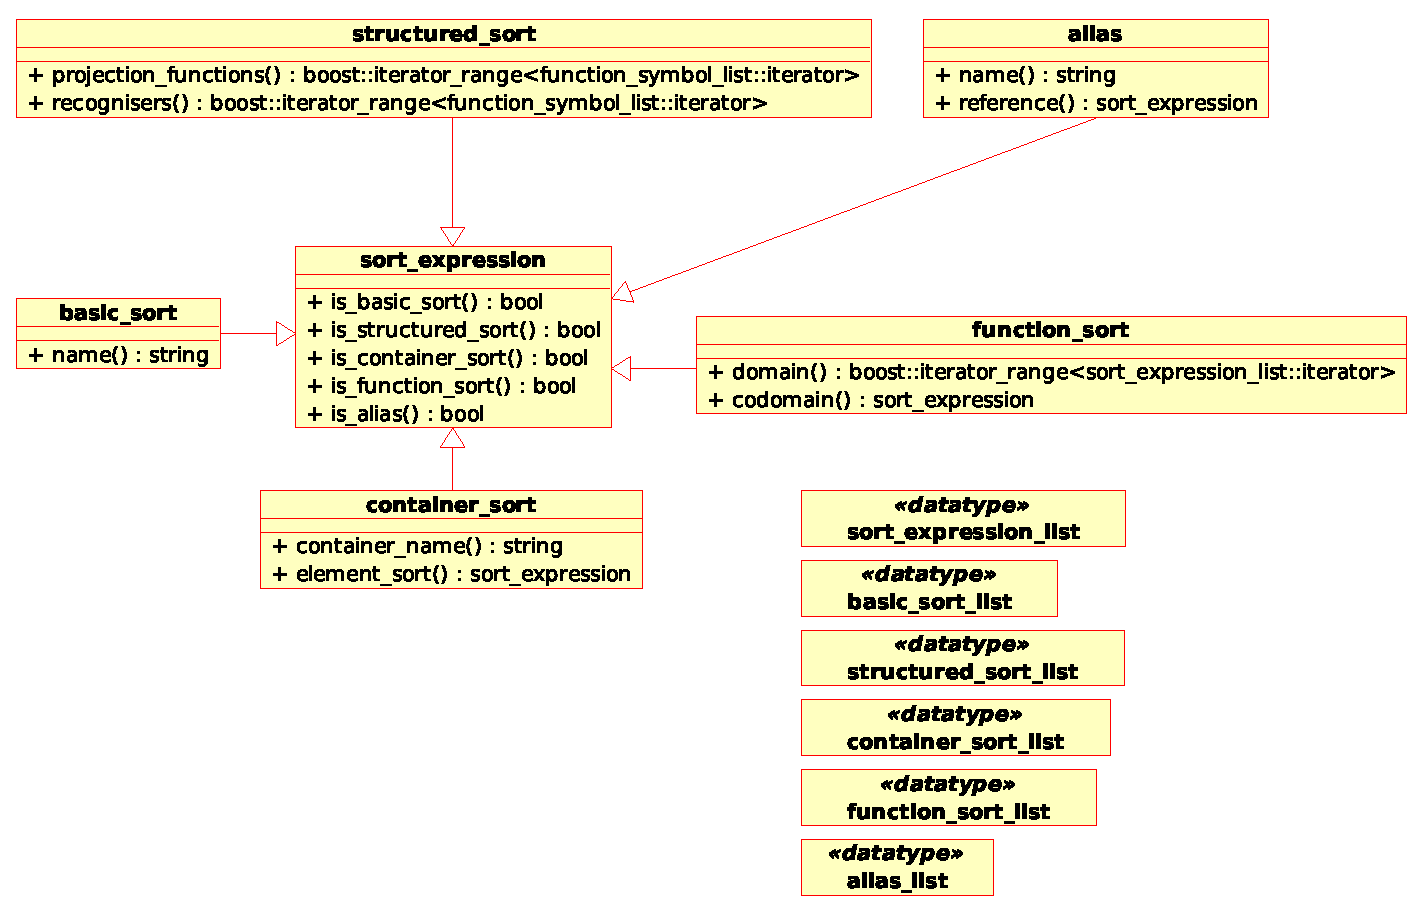
\includegraphics[width=\textwidth]{sort_expr}
      \caption{Class model for the sort expressions (in namespace \texttt{data})}
      \label{fig:class_sort_expr}
    \end{center}
  \end{figure}

\subsubsection{Classes}
We provide an overview of the classes with a short description, we also describe their public methods: 

\dataclass
  {sort\_expression}
  {This denotes any sort expression that can be constructed from the theory, hence any sort occurring in the signature of a specification.}
  {}
  {\begin{itemize}
    \item basic\_sort
    \item structured\_sort
    \item container\_sort
    \item function\_sort
   \end{itemize}}
  {\begin{description}
    \item[is\_basic\_sort] Returns \true iff this expression is a basic sort.
    \item[is\_structured\_sort] Returns \true iff this expression is a structured sort.
    \item[is\_container\_sort] Returns \true iff this expression is a container sort.
    \item[is\_function\_sort] Returns \true iff this expression is a function sort.
   \end{description}}


\dataclass
  {basic\_sort}
  {This represents a basic sort, corresponding directly to the theory.}
  {sort\_expression}
  {}
  {\begin{description}
    \item[name] Returns the name of the basic sort.
   \end{description}}


\dataclass
  {function\_sort}
  {This denotes a function sort $S_0 \times ... \times S_n \rightarrow S$, where $S_0, \dots, S_n$ is the domain, and S is the codomain.}
  {sort\_expression}
  {}
  {\begin{description}
    \item[domain] Returns the domain of the function sort. The domain of $S_0 \times \dots \times S_n \rightarrow S$ is $S_0, \dots, S_n$.
    \item[codomain] Returns the codomain of the function sort. The codomain of $S_0 \times \dots \times S_n \rightarrow S$ is $S$.
   \end{description}}


\dataclass
  {alias}
  {This denotes an alternative name for a sort, i.e. $S_0 = S_1$.}
  {sort\_expression}
  {}
  {\begin{description}
    \item[name] Returns the name of the alias. For example the name of the alias $S = T$ is $S$.
    \item[reference] Returns the sort the name refers to. For example the reference of the alias $S = T$ is $T$.
   \end{description}}


\dataclass
  {structured\_sort}
  {This denotes a structured sort
   \begin{eqnarray*}
     \textbf{struct} & c_1(pr_{1,1}:S_{1,1}, \dots, pr_{1,k_1}:S_{1,k_1})?isc_1\\
                 \mid & c_2(pr_{2,1}:S_{2,1}, \dots, pr_{2,k_2}:S_{2,k_2})?isc_2\\
                 \mid & \vdots\\
                 \mid & c_n(pr_{n,1}:S_{n,1}, \dots, pr_{n,k_n}:S_{n,k_n})?isc_n;
    \end{eqnarray*}
    where $c_1, \dots, c_n$ are called the constructors. In the sequel, where we write $Struct_{example}$, this entire structured sort should be substituted.

    $pr_{i,j}$ are called the projection functions. Note that the sort of projection function function $pr_{i,j}$ is $Struct_{example} \rightarrow S_{i,j}$. $isc_i$ are called recogniser functions. The sort of recogniser function $isc_i$ is $Struct_{example} \rightarrow Bool$}
  {sort\_expression}
  {}
  {\begin{description}
    \item[projection\_functions] Returns the projection functions of the structured sort.
    \item[recognizers] Returns the recogniser functions of the structured sort.
    \item[structured\_sort\_constructors] Returns the constructors of the structured sort, including the projection and recogniser functions.
   \end{description}}


\dataclass
  {container\_sort}
  {This represents container sorts. These are sorts with a name and an element sort. An example of this is $\List(Nat)$, representing the List of natural numbers. In this, List is the name of the container, and Nat is the element sort.}
  {sort\_expression}
  {}
  {\begin{description}
    \item[container\_name] Returns the name of the container. For example the container name of $\List(Nat)$ is $List$.
    \item[element\_sort] Returns the sort of the elements of the container. For example the element sort of $\List(Nat)$ is $Nat$.
   \end{description}}


%  \item[sort\_visitor] is an abstract visitor class. This can be used by concrete visitors to implement operations on sorts. For an in-depth explanation of the visitor pattern see also \cite{gamma94dp}.

\subsubsection{Lists of sorts}
For all classes concerned with sorts, list types are proved of the form $class\_list$. This amounts to the following types:
\begin{description}
 \item[sort\_expression\_list] List of sort expressions
 \item[basic\_sort\_list] List of basic sorts
 \item[structured\_sort\_list] List of structured sorts
 \item[container\_sort\_list] List of container sorts
 \item[function\_sort\_list] List of function sorts
 \item[alias\_list] List of aliases
%  \item[list\_sort\_list] List of list sorts
%  \item[set\_sort\_list] List of set sorts
%  \item[bag\_sort\_list] List of bag sorts
\end{description}

All these list types provide iterator interfaces.

\FloatBarrier
\subsection{Data expressions}
% \comment{Open questions:
% \begin{itemize}
%  \item How do we best treat system defined data expressions (like \&\&:BoolxBool->Bool). Possibilities are having them explicitly as subclass of data\_expression, or creating convenience functions for them at data\_specification level.
%  \item Should we treat forall, exists, where, set/bag comprehension/enumeration the same as system defined functions like and,or?
% \end{itemize}
% }
% 
% \comment{TODO:
% \begin{itemize}
%  \item Add constructors
%  \item Add setters/getters
% \end{itemize}
% }

\begin{figure}[htp]
    \begin{center}
      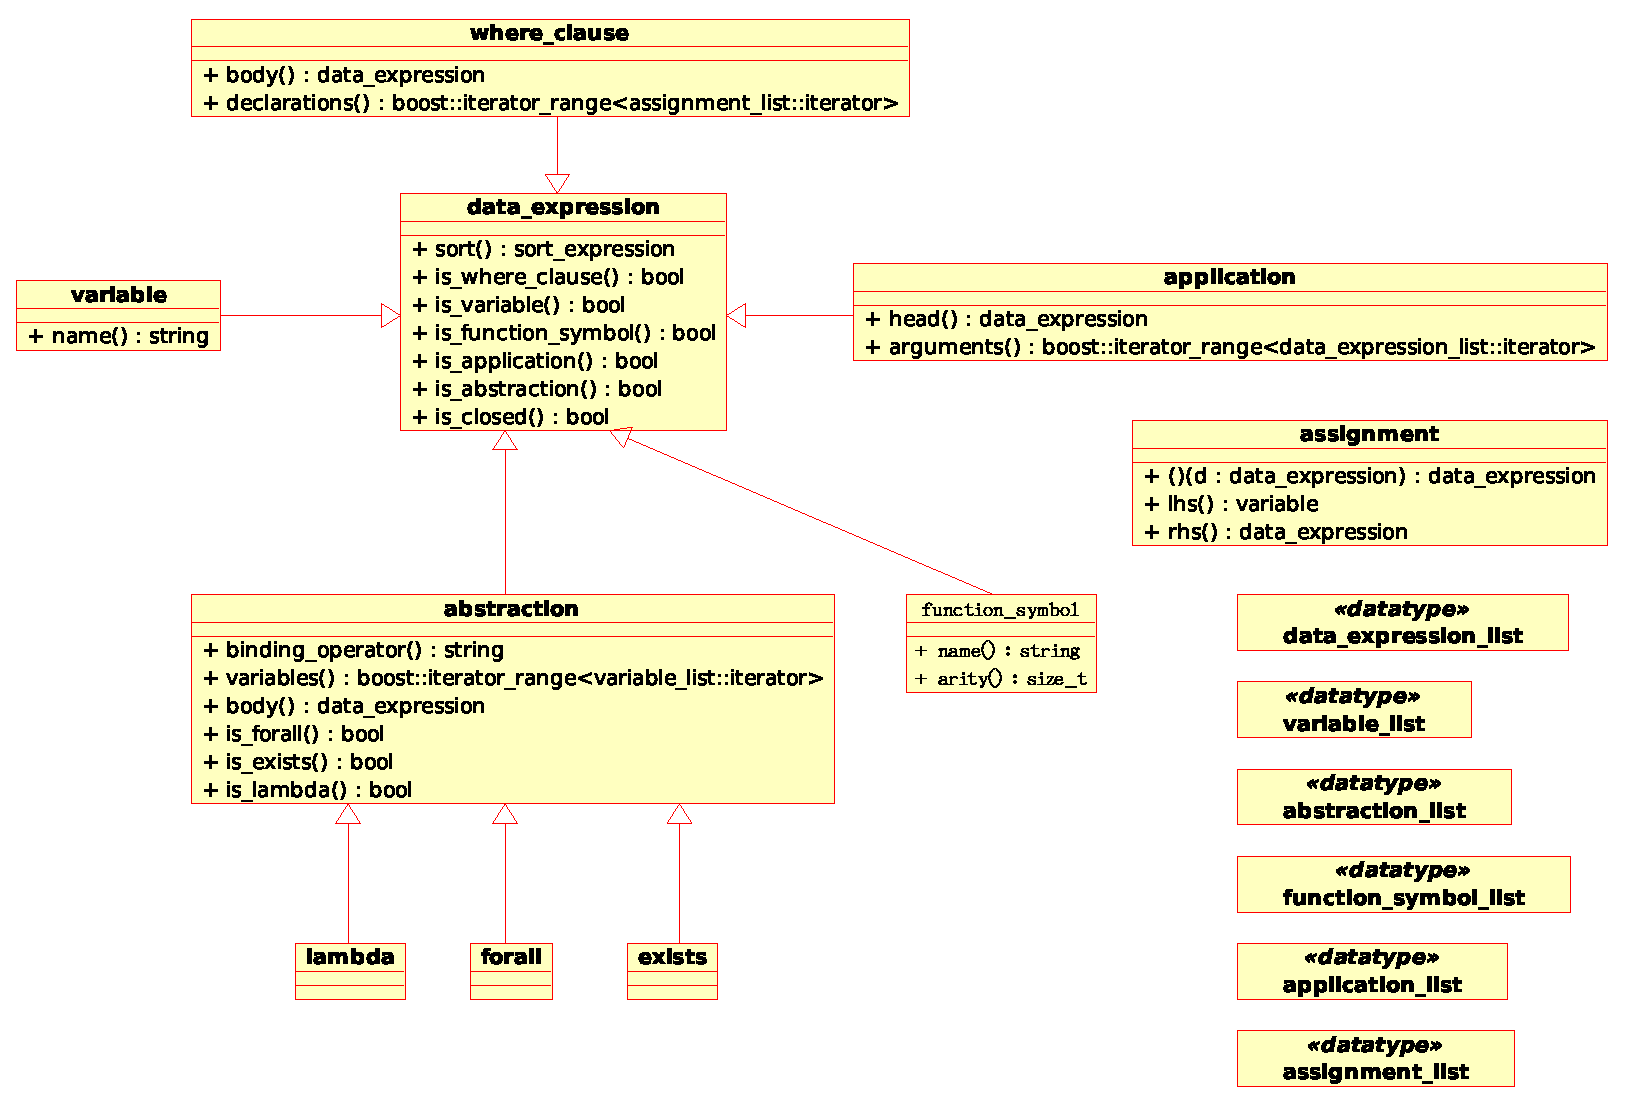
\includegraphics[width=\textwidth]{data_expr}
      \caption{Class model for the data expressions (in namespace \texttt{data})}
      \label{fig:class_data expressions}
    \end{center}
  \end{figure}

\subsubsection{Classes}

% \begin{tabular}{p{3cm} p{11cm}}
%  \hline
%  \multicolumn{2}{c}{\textbf{data\_expression}} \\\hline \hline
%  \textbf{description} & {This denotes a data expression. The date expression structure corresponds directly to the definition in the theory} \\\hline
%  \textbf{subclass of} &\\\hline
%  \textbf{superclass of} &
%     variable, function\_symbol, application, abstraction, where\_clause, set\_comprehension,  bag\_comprehension, set\_enumeration, bag\_enumeration \\\hline
%  \textbf{public methods} &
%     \textbf{sort} Returns the sort of the data expression.\\&
%     \textbf{is\_variable} Returns \true iff the data expression is a variable.\\&
%     \textbf{is\_function\_symbol} Returns \true iff the data expression is a function symbol.\\&
%     \textbf{is\_abstraction} Returns \true iff the data expression is an abstraction.\\&
%     \textbf{is\_application} Returns \true iff the data expression is an application.\\&
%     \textbf{is\_where\_clause} Returns \true iff the data expression is a where clause.\\&
%     \textbf{is\_set\_comprehension} Returns \true iff the data expression is a set comprehension.\\&
%     \textbf{is\_bag\_comprehension} Returns \true iff the data expression is a bag comprehension.\\&
%     \textbf{is\_set\_enumeration} Returns \true iff the data expression is a set enumeration.\\&
%     \textbf{is\_set\_enumeration} Returns \true iff the data expression is a set enumeration.\\\hline
% \end{tabular}

\dataclass
  {data\_expression}
  {This denotes a data expression. The data expression structure corresponds directly to the definition in the theory. }
  {}
  {\begin{itemize}
    \item variable
    \item function\_symbol
    \item application
    \item abstraction
    \item where\_clause
   \end{itemize}}
  {\begin{description}
    \item[sort] Returns the sort of the data expression.
    \item[is\_variable] Returns \true iff the data expression is a variable.
    \item[is\_function\_symbol] Returns \true iff the data expression is a function symbol.
    \item[is\_abstraction] Returns \true iff the data expression is an abstraction.
    \item[is\_application] Returns \true iff the data expression is an application.
    \item[is\_where\_clause] Returns \true iff the data expression is a where clause.
    \item[is\_closed] Returns \true iff the data expression is closed.
   \end{description}}


\dataclass
  {variable}
  {This denotes a variable.}
  {data\_expression}
  {}
  {\begin{description}
    \item[name] Returns the name of the variable.
   \end{description}}


\dataclass
  {function\_symbol}
  {This denotes function symbols.}
  {data\_expression}
  {}
  {\begin{description}
    \item[name] Returns the name of the function symbol.
    \item[arity] Returns the arity of this function.
   \end{description}}


\dataclass
  {abstraction}
  {This denotes lambda abstraction. Body is the data expression which is abstracted from, variables contains the abstraction variables.}
  {data\_expression}
  {\begin{itemize}
    \item lambda
    \item forall
    \item exists
   \end{itemize}}
  {\begin{description}
    \item[binding\_operator] Returns the binding operator of the abstraction.
    \item[variables] Returns the binding variables of the abstraction. Note that this is never empty.
    \item[body] Returns the body of the abstraction, i.e. the expression that is abstracted.
    \item[is\_lambda] Returns \true iff the abstraction is a lambda abstraction.
    \item[is\_forall] Returns \true iff the abstraction is a universal quantification.
    \item[is\_exists] Returns \true iff the abstraction is an existential quantification.
   \end{description}}


\dataclass
  {application}
  {This denotes application of a data expression (head) to a number of other data expressions (arguments).}
  {data\_expression}
  {}
  {\begin{description}
   \item[head] Returns the head of the application. For example the head of $t(t_0, \dots, t_n)$ is $t$.
   \item[arguments] Returns the arguments of the application. For example the arguments of $t(t_0, \dots, t_n)$ are $t_0, \dots, t_n$.
  \end{description}}


\dataclass
  {lambda}
  {This denotes lambda abstraction. This is an abstraction with binding operator lambda.}
  {abstraction}
  {}
  {}


\dataclass
  {forall}
  {This denotes universal quantification. This is an abstraction with binding operator forall.}
  {abstraction}
  {}
  {}


\dataclass
  {exists}
  {This denotes existential quantification. This is an abstraction with binding operator exists.}
  {abstraction}
  {}
  {}

\dataclass
  {where\_clause}
  {This denotes a where clause, e.g. $e \textbf{~whr~} x_0 = e_0, \dots x_n = e_n$. Note that this behaves as a beta redex.}
  {data\_expression}
  {}
  {\begin{description}
   \item[body] Returns the body of the where clause.
   \item[declarations] Returns the local declarations of the where clause.
  \end{description}}


\dataclass
  {assignment}
  {This describes an assignment of a value (data expression) to a data variable.}
  {}
  {}
  {\begin{description}
    \item[()(d)] Returns $d$ in which the assignment has been applied.
    \item[lhs] Returns the variable which is assigned a value.
    \item[rhs] Returns the data expression which is assigned to the variable.
   \end{description}}

%   \item[data\_expression\_visitor] is an abstract visitor class. This can be used by concrete visitors to implement operations on data expressions.

\subsubsection{Lists of data expressions}
For all classes concerned with data expressions, list types are proved of the form $class\_list$. This amounts to the following types:
\begin{description}
 \item[data\_expression\_list] List of data expressions
 \item[variable\_list] List of variables
 \item[abstraction\_list] List of abstractions
 \item[function\_symbol\_list] List of function symbols
 \item[application\_list] List of applications
 \item[assignment\_list] List of assignments
\end{description}

All these list types provide iterator interfaces.

\FloatBarrier
\subsection{Data specification}
A data specification represents a signature $\Sigma$ with an associated set of equations $E$.

\begin{figure}[htp]
    \begin{center}
      
\includegraphics[width=\textwidth]{specification}
      \caption{Class model for the data specification (in namespace \texttt{data})}
      \label{fig:class_specification}
    \end{center}
  \end{figure}

\subsubsection{Classes}

\dataclass
  {data\_specification}
  {This represents a data specification, directly from the theory. Note that sort aliases are included in the specification explicitly.\footnote{Note that additional methods may be added as the need arises.}}
  {}
  {}
  {\begin{description}
    \item[sorts] Returns all sorts in the specification, except the function sorts.
    \item[constructors] Returns all constructors declared in the specification.
    \item[mappings] Returns all mappings declared in the specification.
    \item[equations] Returns all equations declared in the specification.
    \item[aliases(s)] Returns all aliases of sort $s$.
    \item[dependent\_sorts(constructor)] Returns all sorts on which a constructor depends. See also Section~\ref{sec:sort_finiteness}.
    \item[dependent\_sorts(sort)] Returns all sorts on which a sort depends. See also Section~\ref{sec:sort_finiteness}.
    \item[constructors(sort)] Returns all constructors of $sort$.
    \item[mappings(sort)] Returns all mappings which have $sort$ as a result.
    \item[equations(d)] Returns all equations with $d$ as the head of one of its sides.
    \item[is\_certainly\_finite(s)] Returns true iff sort $s$ is definately finite.
    \item[default\_expression] Returns a valid data expression according to this data specification of the given sort s. If no valid expression can be found, an exception is thrown. It returns a minimal term. When selecting function symbols, constructor symbols have a preference over mappings. For each sort, the same term is returned.
    \item[add\_sort] Adds a sort to the specification.
    \item[add\_alias] Adds an alias, so a name for a (possibly new) sort to the specification.
    \item[add\_constructor] Adds a constructor to the specification.
    \item[add\_mapping] Adds a mapping to the specification.
    \item[add\_equation] Adds an equation to the specification.
    \item[add\_sorts(sl)] Adds all sorts in $sl$ to the specification.
    \item[add\_constructors(fl)] Adds all constructors in $fl$ to the specification.
    \item[add\_mappings(fl)] Adds all mappings in $fl$ to the specification.
    \item[add\_equations(el)] Adds all equations in $el$ to the specification.
   \end{description}}


\dataclass
  {data\_equation}
  {This represents a conditional equation, in which variables may be used.}
  {}
  {}
  {\begin{description}
    \item[variables] Return the variables from the variable declaration section of the data equation.
    \item[condition] Returns the condition of the equation.
    \item[lhs] Returns the left hand side of the equation.
    \item[rhs] Returns the right hand side of the equation.
   \end{description}}

\subsubsection{Lists}
In addition to the lists defined so far, we also have the following list:
\begin{description}
 \item[data\_equation\_list] A list of data equations.
\end{description}

\FloatBarrier
\subsection{Utilities}
This section describes a number of utilities for simplifying data expressions, and deciding equality. Note that this section merely describes minimal interfaces the actual components should adhere to.

\begin{figure}[htp]
    \begin{center}
      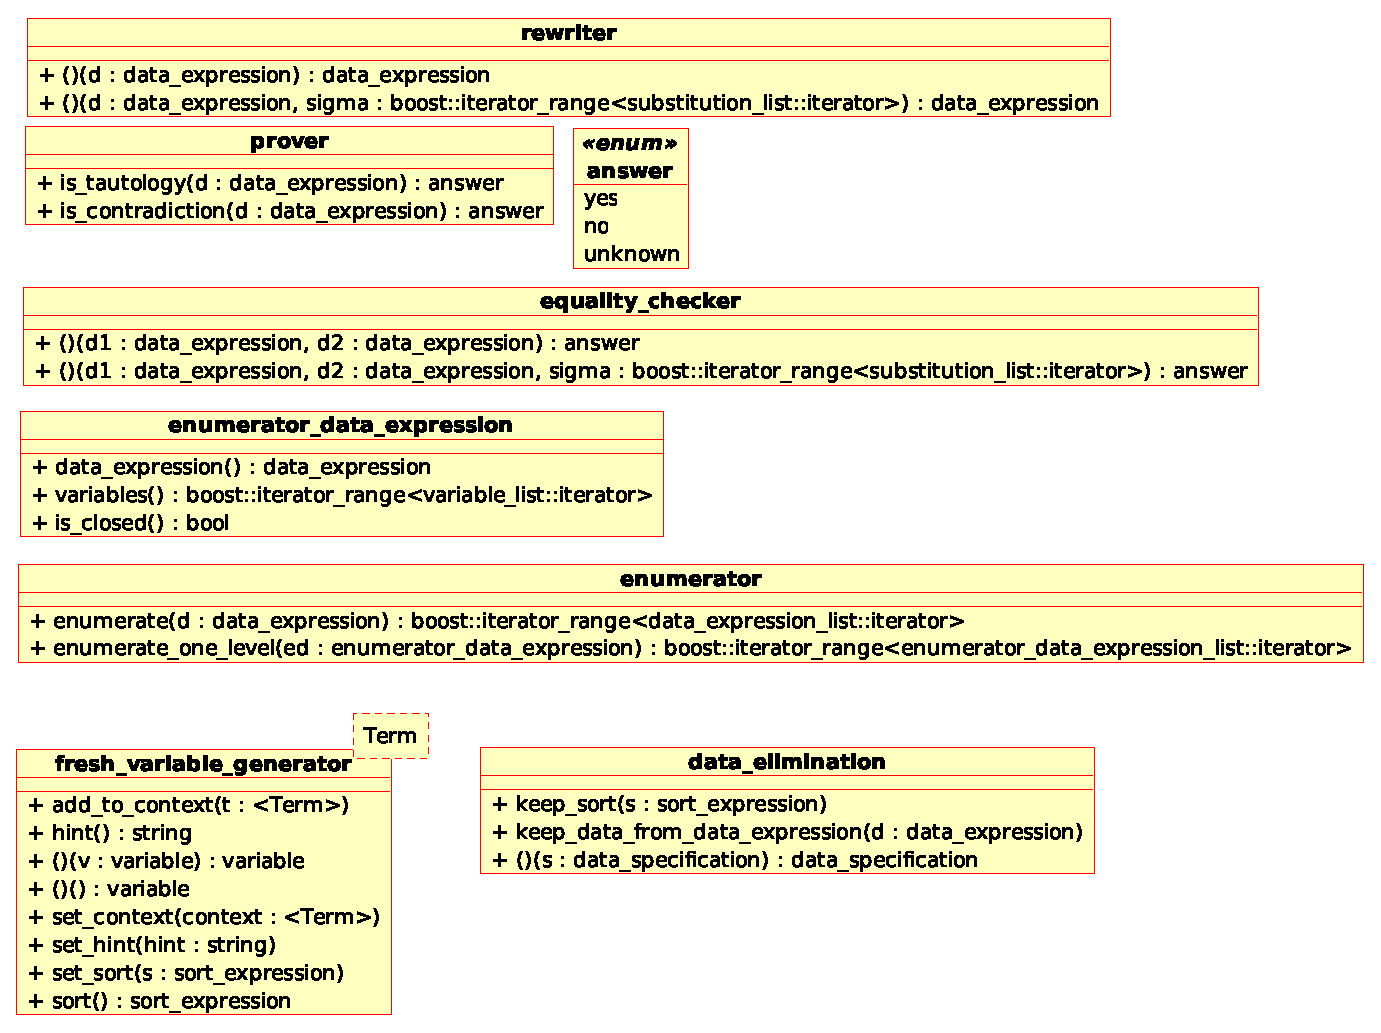
\includegraphics[width=\textwidth]{utilities}
      \caption{Class model for the utilities (in namespace \texttt{data})}
      \label{fig:class_utilities}
    \end{center}
  \end{figure}

\subsubsection{Classes}

\dataclass
  {rewriter}
  {A rewriter uses the equations from a data specification to obtain a normal form for a data expression. Upon construction time of the rewriter object a data specification is provided.}
  {}
  {}
  {\begin{description}
    \item[()(d)] returns the normal form of $d$
    \item[()(d, sigma)] returns the normal form of $d$. On the fly the substitutions in $sigma$ are performed. This is a variant of the rewriter which allows for more efficient rewriting in some cases.
   \end{description}}


\dataclass
  {enumerator\_data\_expression}
  {Contains a data expression which should be enumerated, and the variables that should be expanded}
  {}
  {}
  {\begin{description}
    \item[data\_expression] Gives the data expression it contains.
    \item[variables] Gives the variables to be expanded.
    \item[is\_closed] Returns $true$ if the data expression is closed.
   \end{description}}


\dataclass
  {enumerator}
  {An enumerator returns the set of all possible values that a term can attain.}
  {}
  {}
  {\begin{description}
    \item[enumerate(d)] Gives the set of all possible values that $d$ can attain.
    \item[enumerate\_one\_level(ed)] Gives the set resulting from expanding all variables of $ed$ in the data expression of $ed$ exactly once.
   \end{description}}


\dataclass
 {equality\_checker}
 {Determines whether two expressions are equal. If equality cannot be decided, false is returned.}
 {}
 {}
 {\begin{description}
   \item[()(t,t')] Returns $yes$ if $t$ and $t'$ are equal, $no$ if they are not equal, $unknown$ otherwise.
   \item[()(t,t', sigma)] Returns $yes$ if $t$ and $t'$ are equal under substitution $sigma$, $no$ if they are not equal under $sigma$, $unknown$ otherwise.
  \end{description}}


\dataclass
  {prover}
  {A prover determines whether a boolean expression is either a tautology or a contradiction. Note that it may be the case that a formula is neither a tautology, nor a contradiction.}
  {}
  {}
  {\begin{description}
    \item[is\_tautology(d)] Returns $yes$ if data expression $d$ is a tautology, $no$ if $d$ is not a tautology, $unknown$ otherwise.
    \item[is\_contradiction(d)] Returns $yes$ if data expression $d$ is a contradiction, $false$ if $d$ is not a contradiction, $unknown$ otherwise.
   \end{description}}

\dataclass
  {fresh\_variable\_generator}
  {Generates variables with names that do not appear in the given context.}
  {}
  {}
  {\begin{description}
    \item[add\_to\_context] Adds a term to the context.
    \item[hint] Returns the current hint that is used in the generated variable name.
    \item[()(v)] Returns a fresh variable of the same sort as $v$ using the name of $v$ as hint.
    \item[()()] Returns a fresh variable of sort $sort$ using $hint$.
    \item[set\_context] Sets the context to given term.
    \item[set\_hint] Sets the hint.
    \item[set\_sort] Sets the sort of the variables to be generated.
    \item[sort] Returns the current sort of variables that are generated.
   \end{description}}

\dataclass
  {data\_eliminator}
  {Facilitates elimination of unused or unnecessary parts of a data specification.}
  {}
  {}
  {\begin{description}
    \item[keep\_sort] Keep the sort, and all sorts it depends on.
    \item[keep\_data\_from\_data\_expression] Keep the sorts and mappings used in data expression.
    \item[()] Remove all sorts and data expressions that should not be kept from the data specification.
   \end{description}}


\subsubsection{Lists}
For the classes in utilities we also have lists, with their corresponding iterators:
\begin{description}
 \item[enumerator\_data\_expression\_list] A list of enumerator data expressions.
\end{description}

\subsubsection{Type definitions}
In order to denote that an answer is unknown in the equality checker and the prover we introduce a tri-valued type \textbf{answer} with the obvious meaning.

\subsubsection{Utility functions}
There are also a number of utility functions in the data library that are plain functions. These will be described in this section.

\paragraph{find}
First of all there are a number of find functions which follow the find functions in the details section of the current data library. We will only give their names here.

\begin{description}
  \item[find\_data\_expression]
  \item[find\_data\_variable]
  \item[find\_data\_application]
  \item[find\_function\_symbol]
  \item[find\_abstraction]
  \item[find\_all\_data\_expressions]
  \item[find\_all\_data\_variables]
  \item[find\_all\_data\_applications]
  \item[find\_all\_function\_symbols]
  \item[find\_all\_abstractions]
  \item[find\_sort\_expression]
  \item[find\_basic\_sort]
  \item[find\_structured\_sort]
  \item[find\_container\_sort]
  \item[find\_alias]
  \item[find\_all\_sort\_expressions]
  \item[find\_all\_basic\_sorts]
  \item[find\_all\_structured\_sorts]
  \item[find\_all\_container\_sorts]
  \item[find\_all\_aliases]
\end{description}

\paragraph{replace}
Additionally there are a number of functions to facilitate replacements. Again this follows the same pattern as in the current implementation, and we provide reference to the names only.

\begin{description}
  \item[replace\_data\_expressions]
  \item[replace\_data\_variables]
  \item[replace\_basic\_sorts]
  \item[replace\_sort\_expressions]
\end{description}

\subsection{System defined functions and equations}
For each system defined sort, i.e. $Bool$, $Pos$, $Nat$, $Int$ and $Real$, utility functions will be created to add the declarations of these sorts, with their constructors, mappings and equations to a data specification. For other system defined mappings and equations similar functions will be constructed. Note that for everything that is added in this way, it is recorded that it is system defined. Furthermore utility functions will be added to facilitate easy manipulation of these system defined sorts.

\bibliography{references}

% \paragraph{Class name}
% \subparagraph{description}
%
% \subparagraph{superclass of}
%
% \subparagraph{subclass of}
%
% \subparagraph{public methods}
% \begin{description}
%  \item
% \end{description}

\end{document}

